\section{五}

\subsection{五法}
此在《瑜伽師地論》、《顯揚聖教論》、《成唯識論》、《佛性論》等均有說到。
\begin{enumerate}
  \item 名─事物的名稱
  \item 相─由名而浮起的想像
  \item 分別─對名與相的判斷
  \item 正智─是看破名相為非實的智慧
  \item 如如─作為智慧對象的平等真如
\end{enumerate}
此五法是舉迷界的主觀(分別)客觀(名、相),及悟界的主觀(正智)客觀(如如),而打破迷界以進入悟界的經過,分作五個階段來考察之意。



\subsection{五蘊}
佛教借用五蘊來分析此精神和物質
\paragraph{五蘊即是物與心的配合}
第一色蘊是物理和生理的分析,後四蘊是心理的分析。
以物理、生理、心理的分析,即說明了人生界及宇宙界的一切現象,無一不是無常的、無我的、苦的。
若能證得此中道理,正作如是觀察之時,即是涅槃境界。
\paragraph{眾生的流轉生死} 是由於十二因緣的因緣促成;眾生的身心世界,是由於五蘊的因緣假合。
離了十二因緣,沒有生死流轉;離了五蘊假合,沒有身心世界。生死也好,身心也好,無非是因緣所生的,暫有幻現的虛妄法。
如何勘破它?請用\textbf{三法印}。如何斷絕它?請修\textbf{八正道}。

\begin{itemize}
  \item 色蘊:人類的生理和外在的物理\footnote{由人的眼、耳、鼻、舌、身,及其所對的色、聲、香、味、觸。色蘊含攝一切物質,包括了形色、彩色、極微色、迥遠色。}
  \item 受蘊:以領納為其功用,近於感覺的狀態。
  \item 想蘊:以取相為其功用,近於知覺及想像作用。
  \item 行蘊:有遷流及造作的功用\footnote{含有時間、空間、思想、行為的狀態;即是對於外境,生起貪、瞋等善惡功能的心理活動。}
  \item 識蘊:以分辨為功用,近於知識之義\footnote{以眼、耳、鼻、舌、身、意,為其所依而稱為六識身,負責對於物境的瞭解分別和記憶等作用,也就是心的本體之異名。}
\end{itemize}


\subsection{五根}
修習佛法的根本所在。
\begin{itemize}
  \item 信根,深信三寶;
  \item 进根,修行不懈,指“四正勤”;
  \item 念根,憶念正法,指“四念處”;
  \item 定根,修習禪定;
  \item 慧根,開發智慧。
\end{itemize}

\subsection{五力}
由五根產生的五種力量。
\begin{itemize}
  \item 信力,堅信真理;
  \item 进力,修四正勤的力量;
  \item 念力,破邪、念正的力量;
  \item 定力,置心一處的能力;
  \item 慧力,產生智慧的能力。
\end{itemize}

\subsection{五蓋}
\begin{itemize}
  \item 貪欲蓋
  \item 瞋恚蓋
  \item 惛眠蓋
  \item 掉悔蓋
  \item 疑蓋
\end{itemize}

\subsection{五下分結}
\begin{itemize}
  \item 身見
  \item 疑
  \item 戒禁取見
  \item 欲貪
  \item 瞋
\end{itemize}

\subsection{五上分結}
\begin{itemize}
  \item 色貪
  \item 無色貪
  \item 慢
  \item 掉舉
  \item 無明
\end{itemize}


\subsection{五业}
有部特別重視「業」說的分析。
業在《阿含》經典,是一種「意志」,如說「業是思」。
到了有部,則將業分為二:1.思業,2.思已業。前者為意業,後者為身、語二業。
又將身語二業各分為二:1.表業,2.無表業。
身表業的「體」是「形色」,語表業的「體」是「聲言」;
無表業是業的餘勢,是留存於行為者心上的一種習慣性或影響力,因此意業即不另立無表業。由業分為二業,配合三業,再分為五業
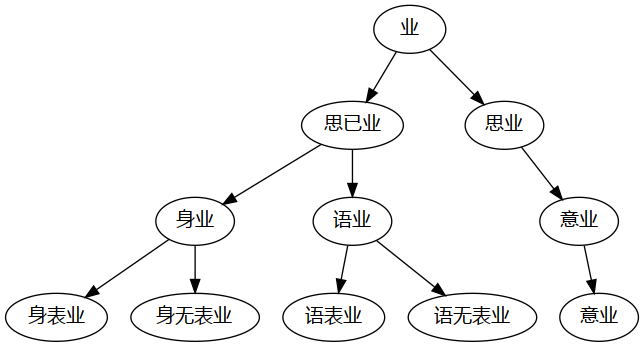
\includegraphics[scale=0.5]{释家/images/五业.png}

\subsection{五無間罪}
\begin{itemize}
  \item 殺父
  \item 殺母
  \item 殺阿羅漢
  \item 破和合僧
  \item 出佛身血
\end{itemize}
